\documentclass[9.5pt]{article}
\usepackage[utf8]{inputenc}
\usepackage[french]{babel}
\usepackage{cvstyle}

\begin{document}

% ---------- Header ----------
\noindent
\begin{minipage}[c]{0.78\textwidth}
  \cvname{Varoujan KARAKOZIAN}\\[2pt]
  \cvrole{Apprenti Ingénieur IA chez Dassault Systèmes}\\[4pt]
  {\small
    +33~7~81~78~53~77 ~~\textbullet~~
    \href{mailto:Varoujan.Karakozian@efrei.net}{Varoujan.Karakozian@efrei.net} ~~\textbullet~~
    3 rue des Œillets, 94140 Alfortville ~~\textbullet~~
    03/11/2005
  }
\end{minipage}%
\hfill
\begin{minipage}[c]{0.15\textwidth}
  \raggedleft
  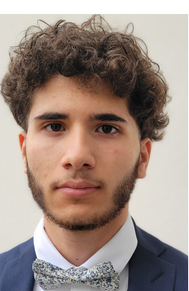
\includegraphics[width=1.85cm]{photo.png}
\end{minipage}

\vspace{2pt}
{\color{accent}\rule{\linewidth}{1.1pt}}
\vspace{2pt}

% ---------- Two-column body ----------
\noindent
\begin{minipage}[t]{0.645\textwidth}

\section*{\large\bfseries\color{accent}Profil}
\vspace{-2pt}
\noindent\small
Apprenti ingénieur en 2\textsuperscript{e} année de cycle ingénieur à l'EFREI Paris, spécialisation \textbf{Big Data \& Machine Learning (BDML)}. En alternance de trois ans (2025--2028) chez \textbf{Dassault Systèmes}, au sein d'une équipe R\&D DevSecOps dédiée à l'assistance IA des développeurs internes, où je développe des outils reposant sur les protocoles \textbf{MCP} et \textbf{RAG}.

\section*{\large\bfseries\color{accent}Formation}
\vspace{-2pt}
\cventry{Cycle Ingénieur, spécialisation Big Data \& Machine Learning}{EFREI Paris (en alternance)}{2025 -- 2028}
{\small 2\textsuperscript{e} année en cours.}

\vspace{2pt}
\cventry{Classe préparatoire intégrée internationale (anglais)}{EFREI Paris}{}

\vspace{2pt}
\cventry{Baccalauréat, mention Bien}{Lycée Sainte-Marie, Créteil}{}

\section*{\large\bfseries\color{accent}Expérience}
\vspace{-2pt}
\cventry{Apprenti Ingénieur IA}{Dassault Systèmes, Vélizy-Villacoublay}{Sept. 2025 -- Juin 2028}
\begin{itemize}\small
  \item Développement d'outils \textbf{MCP} (Model Context Protocol) connectant un assistant de code IA aux systèmes internes : détection automatique du contexte de versionnement, récupération de métadonnées de build, collecte de données via scraping web automatisé (Selenium).
  \item Conception et évaluation d'un pipeline \textbf{RAG} local pour l'indexation de documentation interne (BM25), en remplacement d'une approche basée LLM 2 à 3 ordres de grandeur plus lente et coûteuse en tokens.
  \item Mise en place d'un protocole d'évaluation à trois modèles (génération de questions, réponse, LLM-as-judge) mesurant l'Accuracy@K du retrieval sur environ 8\,500 questions réparties sur 3 corpus.
  \item Contribution à \textbf{FixGen}, un outil d'IA générative de diagnostic de crashs logiciels : développement des outils de collecte de données (classification d'URL, scraping automatisé de stack traces).
\end{itemize}

\vspace{1pt}
\cventry{Stage Commercial}{Lacoste, Créteil}{2025 (1 mois)}
\begin{itemize}\small
  \item Accueil et conseil des clients, recommandations personnalisées adaptées à leurs besoins.
  \item Utilisation de compétences linguistiques (anglais, espagnol) pour conseiller une clientèle étrangère.
\end{itemize}

\vspace{1pt}
\cventry{Stage Ouvrier (préparateur de commande)}{Phoenix Pharma, Créteil}{2024 (1 mois)}
\begin{itemize}\small
  \item Gestion logistique : préparation et vérification de commandes pharmaceutiques.
  \item Travail d'équipe : collaboration efficace avec les équipes d'entrepôt dans un environnement dynamique.
\end{itemize}

\section*{\large\bfseries\color{accent}Projets académiques}
\vspace{-2pt}
\cvproject{NYC Taxi: Data Visualization \& Business Intelligence}{2026}
\begin{itemize}\small
  \item Analyse exploratoire de courses de taxi new-yorkaises (Python, Pandas, Plotly, Streamlit) : nettoyage de données, visualisations interactives, dashboard de BI avec KPIs.
\end{itemize}

\vspace{1pt}
\cvproject{Classification de la qualité du vin : Machine Learning}{2026}
\begin{itemize}\small
  \item Comparaison de plusieurs modèles (Random Forest, SVM, \dots) pour prédire la qualité d'un vin à partir de ses caractéristiques physico-chimiques.
\end{itemize}

\vspace{2pt}
\noindent\small
\textbf{Projets antérieurs :}
\textbf{Analyse du changement climatique} (2025) : ACP de A à Z, corrélation inégalité/pollution nationale.
\textbf{Voll'Effrei} (2025) : jeu vidéo de volley-ball, projet interdisciplinaire physique/informatique.
\textbf{Chatbot intelligent} (2024) : chatbot Python basé sur l'analyse TF-IDF.
\textbf{CDataFrame} (2024) : DataFrame en langage C inspiré de Pandas.

\end{minipage}%
\hfill
\begin{minipage}[t]{0.305\textwidth}

\section*{\large\bfseries\color{accent}Compétences}
\vspace{-2pt}
\small
\textbf{IA / Machine Learning}
\begin{itemize}
  \item MCP (Model Context Protocol)
  \item RAG \& évaluation de RAG
  \item LLM-as-judge, Accuracy@K
  \item BM25, scikit-learn (Random Forest, SVM)
\end{itemize}
\vspace{2pt}
\textbf{Programmation}
\begin{itemize}
  \item Python, C, Java
\end{itemize}
\vspace{2pt}
\textbf{Outils \& plateformes}
\begin{itemize}
  \item Git/GitHub, Linux
  \item Selenium, Streamlit, Plotly, Pandas
\end{itemize}
\vspace{2pt}
\textbf{Bases de données}
\begin{itemize}
  \item SQL, MySQL, SQLite
\end{itemize}
\vspace{2pt}
\textbf{Soft skills}
\begin{itemize}
  \item Travail en équipe
  \item Capacité d'adaptation
  \item Autodidacte
  \item Sens de l'initiative
  \item Créatif
  \item Autonomie
  \item Polyvalent
\end{itemize}

\section*{\large\bfseries\color{accent}Langues}
\vspace{-2pt}
\small
\begin{itemize}
  \item Français : langue maternelle
  \item Anglais : avancé B2
  \item Arménien : intermédiaire B1
  \item Espagnol : intermédiaire B1
\end{itemize}

\section*{\large\bfseries\color{accent}Loisirs}
\vspace{-2pt}
\small
\begin{itemize}
  \item Musique
  \item Escalade
  \item Échecs
  \item Basketball
\end{itemize}

\end{minipage}

\end{document}
